% Template for ICIP-2017 paper; to be used with:
%          spconf.sty  - ICASSP/ICIP LaTeX style file, and
%          IEEEbib.bst - IEEE bibliography style file.
% --------------------------------------------------------------------------
\documentclass{article}
\usepackage{spconf,amsmath,graphicx}
\usepackage{pbox}

% Example definitions.
% --------------------
\def\x{{\mathbf x}}
\def\L{{\cal L}}

% Title.
% ------
\title{AUTHOR GUIDELINES FOR ICIP 2017 PROCEEDINGS MANUSCRIPTS}
%
% Single address.
% ---------------
\name{Author(s) Name(s)\thanks{Thanks to XYZ agency for funding.}}
\address{Author Affiliation(s)}
%
% For example:
% ------------
%\address{School\\
%	Department\\
%	Address}
%
% Two addresses (uncomment and modify for two-address case).
% ----------------------------------------------------------
%\twoauthors
%  {A. Author-one, B. Author-two\sthanks{Thanks to XYZ agency for funding.}}
%	{School A-B\\
%	Department A-B\\
%	Address A-B}
%  {C. Author-three, D. Author-four\sthanks{The fourth author performed the work
%	while at ...}}
%	{School C-D\\
%	Department C-D\\
%	Address C-D}
%
\begin{document}
%\ninept
%
\maketitle
%
\begin{abstract}
The abstract should appear at the top of the left-hand column of text, about
0.5 inch (12 mm) below the title area and no more than 3.125 inches (80 mm) in
length.  Leave a 0.5 inch (12 mm) space between the end of the abstract and the
beginning of the main text.  The abstract should contain about 100 to 150
words, and should be identical to the abstract text submitted electronically
along with the paper cover sheet.  All manuscripts must be in English, printed
in black ink.
\end{abstract}
%
\begin{keywords}
One, two, three, four, five
\end{keywords}
%
\section{Introduction}
\label{sec:intro}
More and more content is being shared everyday on the internet. Most of this content is trivial and does not need to be encrypted. Some of it however needs to be securely transfered, the problem of encryption arises. Full encryption with methods such as AES for exemple are often not needed in addition to not being possible due to computing power constraints. Instead, partial or selective encryption is used, where the goal is sufficient encryption. That is, the image is sufficently distorted and an attacker is not able to access the content. This distortion can be of varying magnitude, a strong distortion for exemple for DRM, or a lighter distortion, where the content is still recognizable to attract the viewers interest. \textit{TODO : encryption state of the art}.

  When an image is intented to be consumed by a human, the most accurate measure of its confidentiality is a Mean Opinion Score, where actual people rate the image. It is however not a realistic way to rate the distortion of an image as it is way to expensive and time consuming, security and quality metrics were introduced as a means to automate the process.

According to \cite{metrics_deficits}, there is not yet a security metric that consistently rates images across all the MOS spectrum. Most quality metrics fail to predict a MOS on low quality images, precisely where it would be most important to do so : decide whether an image is confidential.

We give a quick overview of a few selected metrics. For a more in-depth review, we refer the reader to \cite{metrics_deficits}.

\textbf{PSNR :} Even though it is known that the PSNR is not well correlated with human judgment, it is still widely used due to its speed and ease of use. The range is [0, $+\infty$], where two identical images would have a PSNR of $+\infty$.

\textbf{SSIM :} \cite{ssim}(Structural Similarity Index Measure). A luminance score, au contrast score and a structure score are combined to obtain the actual SSIM score. It has a range of [0;1] where identical images have a score of 1.

\textbf{ESS :} \cite{ess_lss}(Edge Similarity Score). It uses non overlapping 8x8 block directions to compare images. With the range [0;1], a higher score reflects a less distorted image.

\textbf{LSS :} \cite{ess_lss}(Luminance Similarity Score). It uses non overlapping 8x8 block average luminance to compare images. With the range [-8.5, 1] for default parameters of $\alpha=0.1$ and $\beta=3$, a higher score reflects a less distorted image.

\textbf{NPCR :} \cite{npcr_uaci}It is the number of pixel changes between images. Its range is [0,100], where a fully encrypted image has a NPCR close to 100, where almost all the pixels changed.

\textbf{UACI :} \cite{npcr_uaci}It is the unified averaged changed intensity. It is the average intensity difference between two images. Its range is [0,100], where a fully encrypted image has a value close to 33.

\textbf{Entropy :} It is the amount of information in an image, for an 8-bit image, so an entropy of 8 would be the target for a full encryption method. It ranges from 0 to 8 in this case.

\textbf{Correlation :} The correlation coefficient ranges from 0 to 1, it is the average correlation of adjacent pixels in an image, where a natural image would be highly correlated and a fully encrypted image would have low correlation.

\section{Creating the dataset}
\label{sec:dataset}
The cryptocompression method we use is targeted towards JPEG images. We have six parameters that we can enable or not to generate a cryptocompressed image. \textit{Shuffle} and \textit{xor} are the parameters that decide de actual encryption method. \textit{AC} and \textit{DC} control which part of the DCT will be encrypted and two additionnal parameters, \textit{chrominance} and \textit{luminance} decide which of the luminance, chrominance (or both) DCT coefficients will be encrypted. As there must be at least one encryption method, at least one type of coefficient, and chrominance or luminance selected, we have a total of 27 different distortions.

\textbf{Explain shuffle and xor and maybe link Vincent's paper}. We use the training images from the BSDS500 \cite{bsds500} dataset as our input images for a total of $27 * 200 = 5400$ cryptocompressed images.

The 27 distortions are given in Annex \ref{ann:distortions}, they are named according to the parameters enabled and are sorted by MOS, as explained in Section \ref{sec:evaluation}, they are later designated by their number for ease of use.

\section{Image evaluation}
\label{sec:evaluation}
We had a total of \textit{N} different person do the evaluation. They had to give a score from 1 to 5 to the images, where 5 is the best score and 1 is the worst, presented as follows :\\\\
\textbf{1 :} The distortion is unbearable, nothing is visible\\
\textbf{2 :} \small{The distortion is very annoying, I can barely guess the content}\normalsize{}\\
\textbf{3 :} The distortion is annoying, but I can see the content\\
\textbf{4 :} The distortion is slightly annoying, but the content is clear\\
\textbf{5 :} The distortion is not annoying at all \\

They had to rate 81 images, three for every distortion, the sessions were 10 to 15 minutes long, depending on the person. Each image was seen at most once by the user, to prevent them from recognising it giving it a higher score. The distortions order was shuffled differently for every evaluation and repeated three times in the same order. We chose to have every distortion rated three times because during our preliminary tests, we saw that for the first few images, the user was not confident on the score to give to an image, confidence that improved as they saw more images and distortion. It allowed us to filter the outliers caused by the learing curve while still having a good amount of rating.

The images were evaluated in a dim room, on a \textit{details of the screen} screen, about $n$ meters away and around eyes level. The user could only see one image at a time, a new image shown once the previous had been rated.
The MOS obtained during the evaluation are given Fig. \ref{fig:mos}. The name of the distortions are given in Annex \ref{ann:distortions}. We can see that after distortions $17$, the MOS get marginally better, this is due to the absence of the parameter $luminance$, the $shuffle$ and $xor$ are only performed on the chrominance, hence the better ratings.

\begin{figure}[ht]
  \centering
  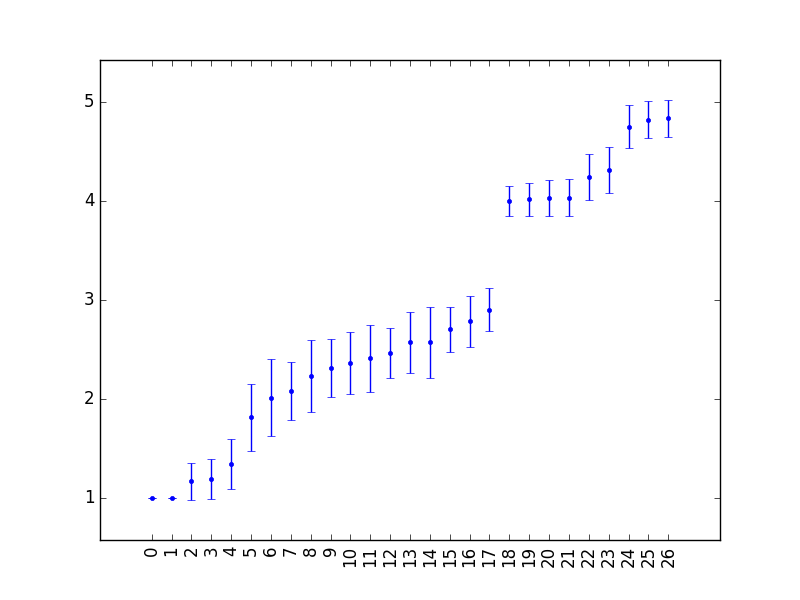
\includegraphics[width=8.5cm]{figures/mos}
  \caption{MOS for the 27 distortions.\label{fig:mos} }
\end{figure}

Our goal is to predict the rating a human would give to an image. In the best case scenario, a metric would be totally correlated with human rating and could be used to completely replace humans in image evaluation, this is however not the case, at least not for the metrics we selected, as shown in figures \ref{fig:psnr},\ref{fig:ssim},\ref{fig:ess},\ref{fig:lss},\ref{fig:npcr},\ref{fig:uaci},\ref{fig:entropy},\ref{fig:correlation}.

\begin{figure}[ht]
  \centering
  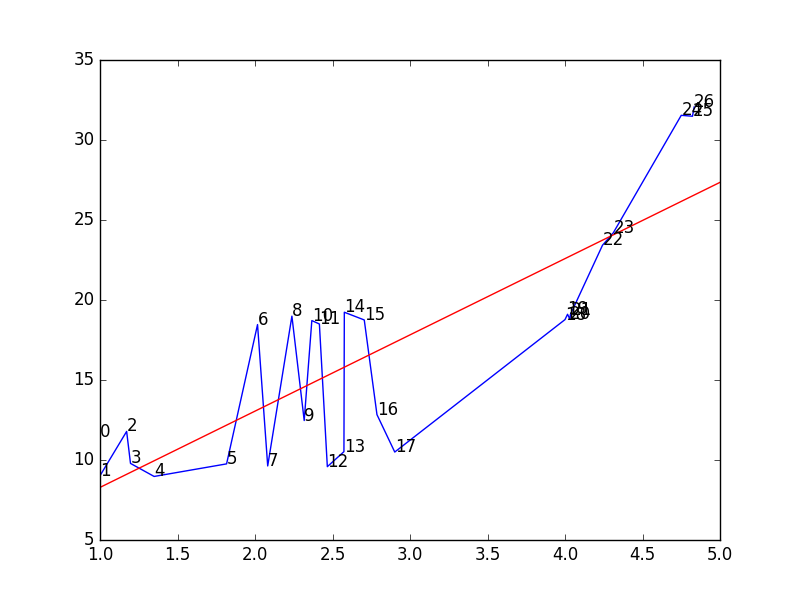
\includegraphics[width=8.5cm]{figures/mos_psnr}
  \caption{MOS on x-axis and PSNR on y-axis\label{fig:psnr} }
\end{figure}
\begin{figure}[ht]
  \centering
  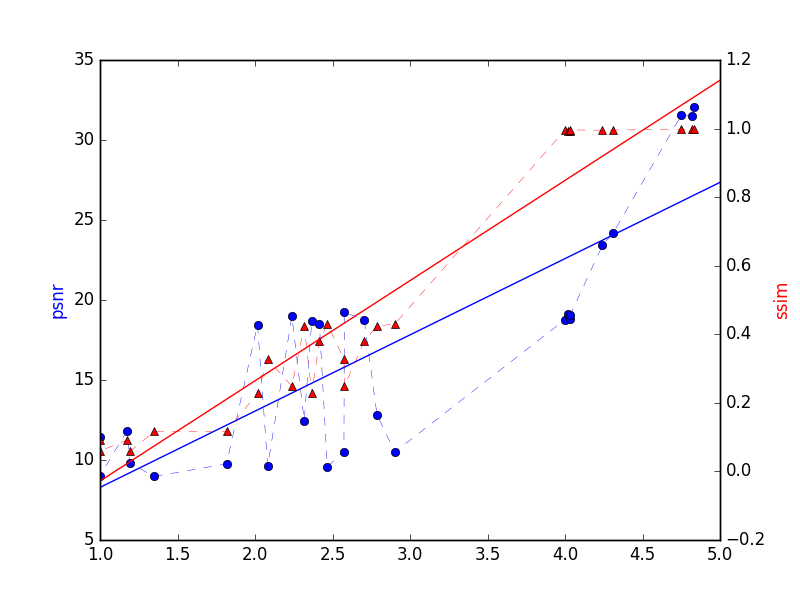
\includegraphics[width=8.5cm]{figures/mos_ssim}
  \caption{MOS on x-axis and SSIM on y-axis\label{fig:ssim} }
\end{figure}
\begin{figure}[ht]
  \centering
  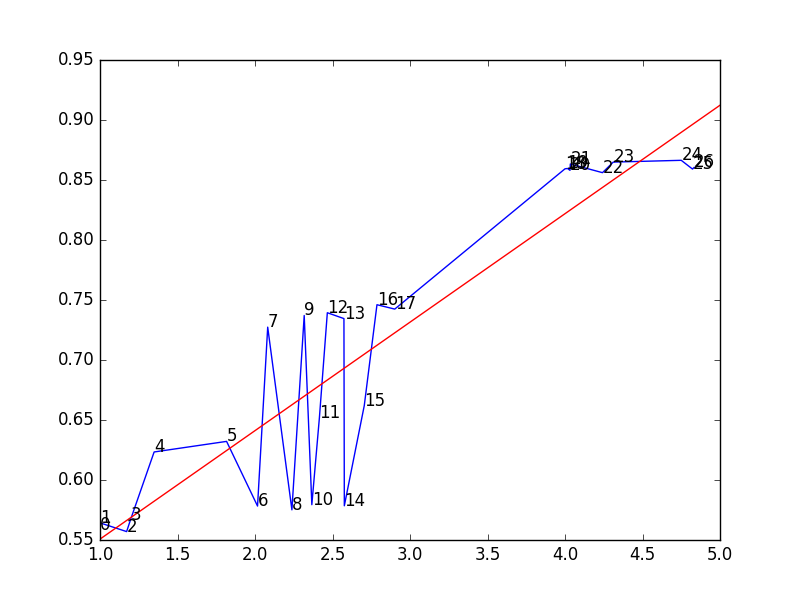
\includegraphics[width=8.5cm]{figures/mos_ess}
  \caption{MOS on x-axis and ESS on y-axis\label{fig:ess} }
\end{figure}
\begin{figure}[ht]
  \centering
  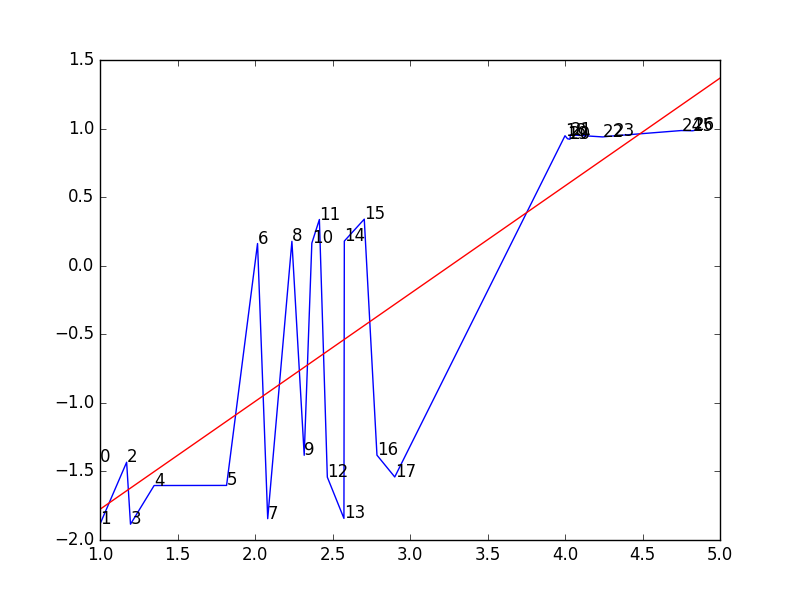
\includegraphics[width=8.5cm]{figures/mos_lss}
  \caption{MOS on x-axis and LSS on y-axis\label{fig:lss} }
\end{figure}
\begin{figure}[ht]
  \centering
  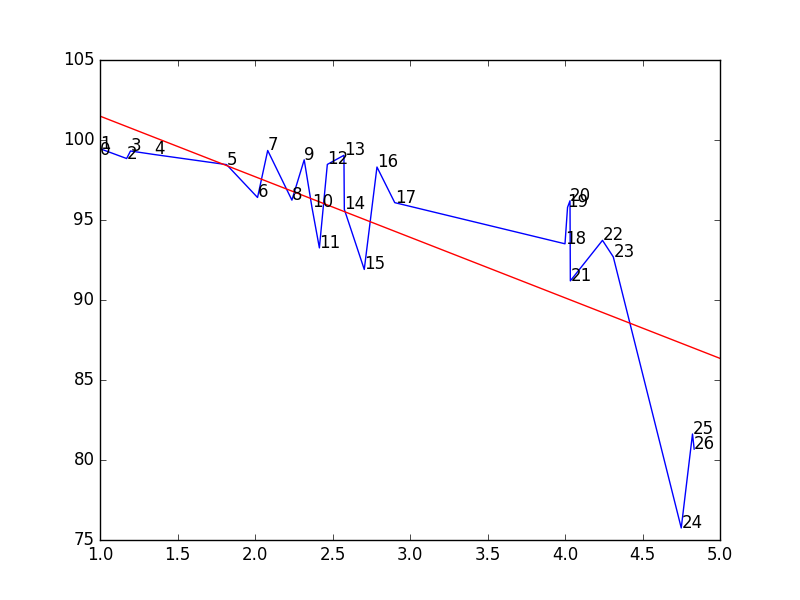
\includegraphics[width=8.5cm]{figures/mos_npcr}
  \caption{MOS on x-axis and NCPR on y-axis\label{fig:npcr} }
\end{figure}
\begin{figure}[ht]
  \centering
  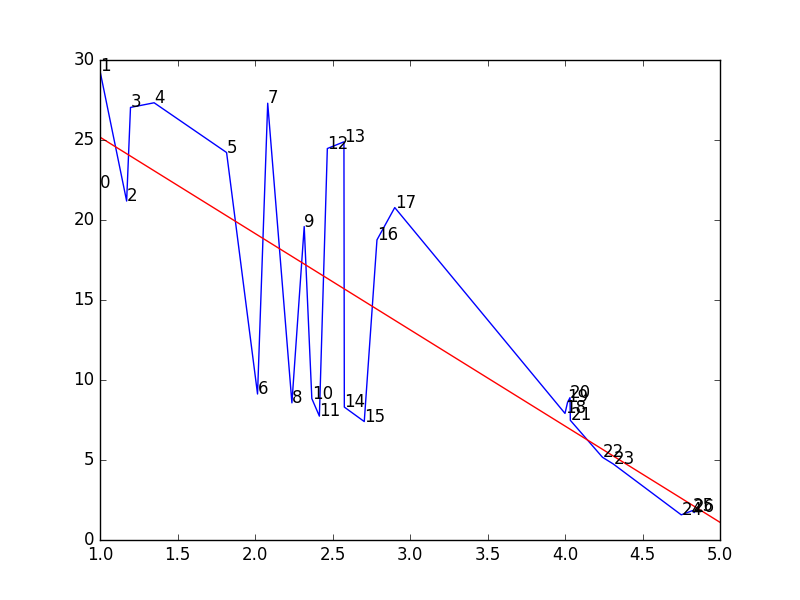
\includegraphics[width=8.5cm]{figures/mos_uaci}
  \caption{MOS on x-axis and UACI on y-axis\label{fig:uaci} }
\end{figure}
\begin{figure}[ht]
  \centering
  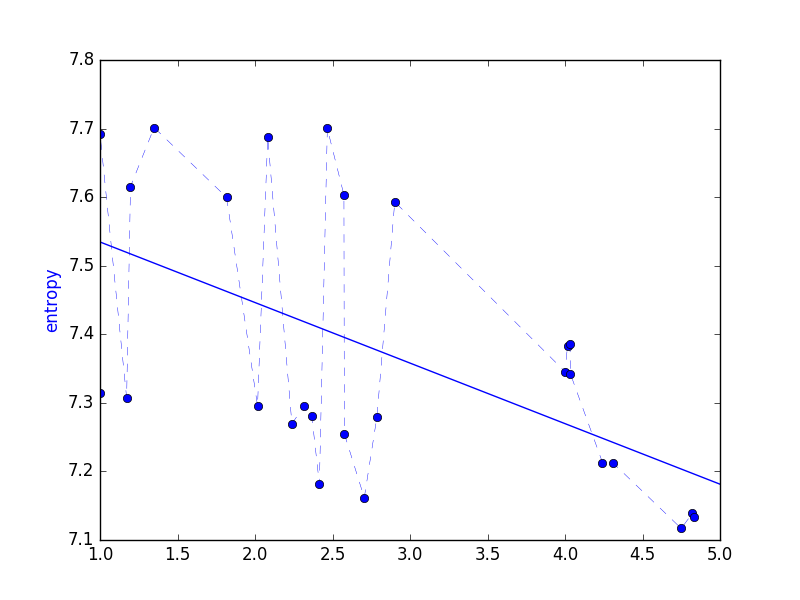
\includegraphics[width=8.5cm]{figures/mos_entropy}
  \caption{MOS on x-axis and entropy on y-axis\label{fig:entropy} }
\end{figure}
\begin{figure}[ht]
  \centering
  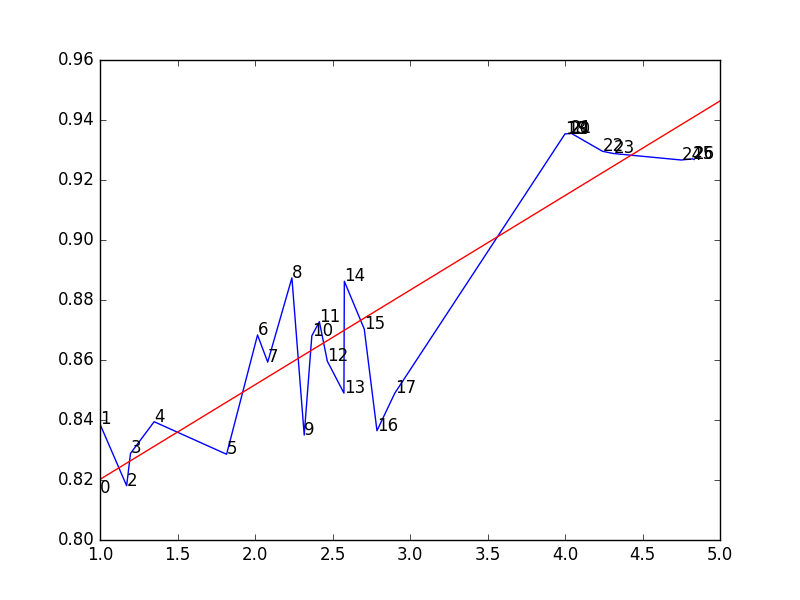
\includegraphics[width=8.5cm]{figures/mos_corr_horiz}
  \caption{MOS on x-axis and horizontal correlation on y-axis\label{fig:correlation} }
\end{figure}
\section{REFERENCES}
\label{sec:ref}

List and number all bibliographical references at the end of the
paper. The references can be numbered in alphabetic order or in
order of appearance in the document. When referring to them in
the text, type the corresponding reference number in square
brackets as shown at the end of this sentence \cite{C2}. An
additional final page (the fifth page, in most cases) is
allowed, but must contain only references to the prior
literature.

% References should be produced using the bibtex program from suitable
% BiBTeX files (here: strings, refs, manuals). The IEEEbib.bst bibliography
% style file from IEEE produces unsorted bibliography list.
% -------------------------------------------------------------------------
\bibliographystyle{IEEEbib}
\bibliography{strings,refs}

\end{document}
